\documentclass{standalone}

\usepackage{tikz}
\usepackage{circuitikz}

\tikzset{block/.style = {draw, fill=white, very thick, rectangle, minimum height=1cm, minimum width=2cm},
         lblock/.style={draw,fill=white,very thick, rectangle, minimum height=3cm, minimum width=1cm},
         sum/.style= {draw, fill=white, very thick, circle, node distance=0.5cm}}

         
\begin{document}
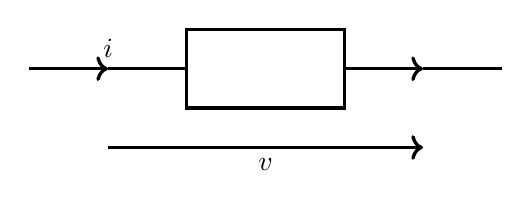
\begin{tikzpicture}[scale=2]
    \node[block](c1)at(3.5,0){};
    \draw[->,very thick](2,0)--(2.5,0)node[above]{$i$};
    \draw[-,very thick](2.5,0)--(c1.180);
    \draw[->,very thick](c1.0)--(4.5,0);
    \draw[-,very thick](4.5,0)--(5,0);
    \draw[<-,very thick](4.5,-0.5)--(2.5,-0.5)node[midway, below]{$v$};
\end{tikzpicture}

\end{document}